% ----------------------------------------------------------
% Subseção Consciência
% ----------------------------------------------------------
\subsection{Consciência}
Um momento lógico pode ser formado por uma divisão (primeiro momento) ou por subdivisões lógicas (demais momentos).
	\begin{figure}[H]
	\caption{Intervalo lógico}
	\label{fig:consciousness_logical_moments}
	\centering
	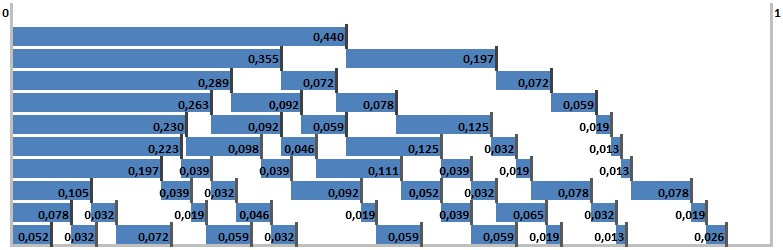
\includegraphics[scale=.7]{sections/images/consciousness_logical_moments.jpg}
	\floatfoot{Exemplo de um intervalo lógico com dez momentos lógicos.}%\footnotemark}
	\end{figure}
	%\footnotetext{Fonte: note}

As unidades de momentos lógicos tendem a formar a maior e mais complexa lógica da população, a maior onda, a consciência.
	\begin{figure}[H]
	\caption{Intervalo lógico consciente}
	\label{fig:consciousness}
	\centering
	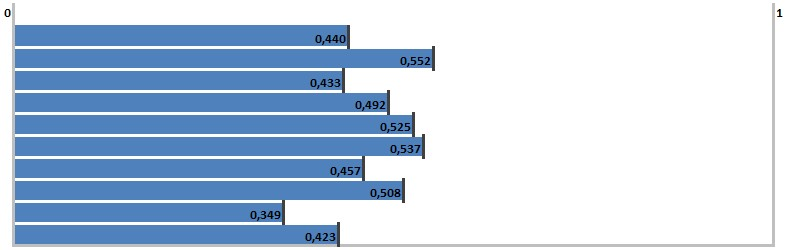
\includegraphics[scale=.7]{sections/images/consciousness.jpg}
	\floatfoot{Exemplo de um intervalo lógico consciente com dez unidades de momentos lógicos.}%\footnotemark}
	\end{figure}
	%\footnotetext{Fonte: note}

Pode ser observado na Tabela \ref{tab:10000_all} que a probabilidade de 99,99\% das amostras de uma população (Amostras do Range), que aumentam em quantidade à medida que crescem os momentos lógicos, tendem a estar cada vez mais ao centro do intervalo lógico, sendo que essa centralização tende ao infinito.
	\begin{figure}[H]
	\caption{Centralização de 99,99\% das amostras}
	\label{fig:centering_of_99_range}
	\centering
	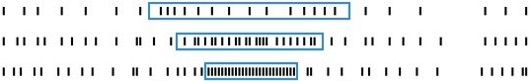
\includegraphics[scale=1]{sections/images/centering_of_99_range.jpg}
	\floatfoot{Tendência de centralização do range de 99,99\% das amostras.}%\footnotemark}
	\end{figure}
	%\footnotetext{Fonte: note}

A maior onda de uma população tende a um histograma da distribuição normal, conforme Figura \ref{fig:trend_chart_of_normal_distribution}. Todos os aspectos listados abaixo são inerentes a abstração lógica chamada consciência.

A primeira amostra de uma população já uma discrepância (um intervalo), logo já se aplica todas as características da consciência, a maior discrepância da população. Desta forma, não há possibilidade de uma expansão populacional que não tenha ao menos uma discrepância. Essa discrepância ou intervalo estará subindo a esquerda, centralizado, a direita ou simultaneamente em qualquer dessas possibilidades, conforme o movimento descrito na subseção do Espaço.

\subsubsection{Infinito}
Um dos aspectos mais importantes que a negação do nada traz (negação de si), é o infinito, ou seja, em qualquer intervalo lógico cabe o infinito novamente. A lógica primordial que iniciou todo o intervalo lógico é a mesma encontrada em seus intervalos subsequentes. Isso fundamenta como uma lógica de alto nível como a subconsciência humana explica a lógica primordial, uma vez que não é preciso voltar ao primeiro momento lógico do intervalo para deduzi-lo, pois esse fenômeno é onipresente em todo o intervalo. Este fenômeno pode ser visto na subseção do Espaço, Plano espacial.

\subsubsection{Ondas}
Probabilisticamente a distribuição de novas amostras de uma população tendem a concentrar mais amostras sentido a mediana da população com frequências de amostras cada vez maiores neste sentido. Porém, a distribuição dessas amostras com frequências de crescimento uniformes é infinitesimal se comparado às possibilidades randômicas desse crescimento. Assim, a tendência de crescimento dessas frequências sentido a mediana somadas a baixíssima probabilidade (infinitesimal) desse crescimento ser uniforme, conduz a frequências no padrão de ondas. A relação de densidade ou amplitude de uma onda com seu comprimento é detalhada subseção posterior.
	\begin{figure}[H]
	\caption{Padrão de onda}
	\label{fig:consciousness_waves}
	\centering
	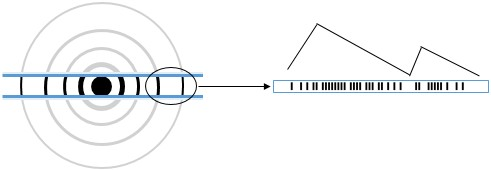
\includegraphics[scale=.8]{sections/images/consciousness_waves.jpg}
	\floatfoot{Padrão de onda inferido pela tendência dessa distribuição com frequências maiores sentido a mediana da população e a baixíssima probabilidade de crescimento uniforme dessas frequências.}%\footnotemark}
	\end{figure}
	%\footnotetext{Fonte: note}

A junção de uma onda a outra elimina sua discrepância e faz com que essa onda deixe de existir a se tornar parte da primeira, que tem seu pico mais próximo da mediana. Uma onda não morre, apenas une-se com outra onda mais ao centro da população.
	\begin{figure}[H]
	\caption{Unificação de ondas}
	\label{fig:consciousness_uniform_wave}
	\centering
	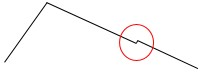
\includegraphics[scale=1]{sections/images/consciousness_uniform_wave.jpg}
	\floatfoot{Ondas sendo unificadas para exemplificar o crescimento amostral uniforme.}%\footnotemark}
	\end{figure}
	%\footnotetext{Fonte: note}

\subsubsubsection{Comprimento e amplitude}
O histograma é utilizado nas figuras dessa subseção e posteriormente para facilitar a visualização e entendimento, pois representa muito bem a curva de densidade de uma população, conforme as diferentes visualizações da Figura \ref{fig:consciousness_wave_histogram} representando apenas um intervalo ou um comprimento de onda pareado pela mediana da população.  
	\begin{figure}[H]
	\caption{Histograma em diferentes visualizações }
	\label{fig:consciousness_wave_histogram}
	\centering
	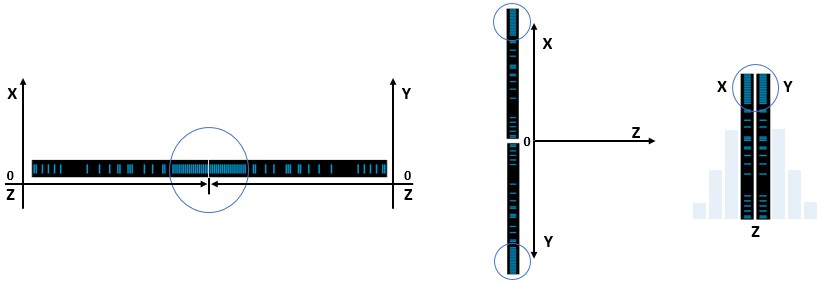
\includegraphics[scale=.7]{sections/images/consciousness_wave_histogram.jpg}
	\floatfoot{Diferentes maneiras da representação populacional em histograma.}%\footnotemark}
	\end{figure}
	%\footnotetext{Fonte: note}}
O comprimento e amplitude de ondas estabelecem uma relação de quantidade por intervalo ou unidade. Essas unidades são estabelecidas pelo entrelaçamento de ondas, conforme subseção posterior. Assim, a amplitude é a densidade de um comprimento de onda, a densidade de um intervalo qualquer.  

Ao adicionar uma nova amostra na população todo o intervalo se distribui proporcionalmente para acoplar essa amostra, conforme Figura \ref{fig:consciousness_space_volume_amplitude}.
	\begin{figure}[H]
	\caption{Expansão do intervalo}
	\label{fig:consciousness_space_volume_amplitude}
	\centering
	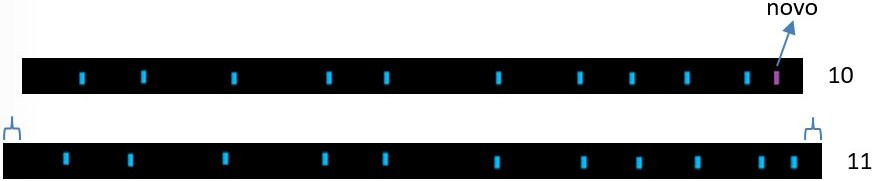
\includegraphics[scale=.5]{sections/images/consciousness_space_volume_amplitude.jpg}
	\floatfoot{Expansão do intervalo com a adição de novas amostras.}%\footnotemark}
	\end{figure}
	%\footnotetext{Fonte: note}}

Em grandes intervalos com muitos momentos lógicos é observado uma discrepância proporcional menor das amplitudes das ondas. Essa característica está relacionada com a maior quantidade de momentos lógicos e possíveis subintervalos que podem compensar e neutralizar mais facilmente os desnivelamentos probabilísticos do intervalo. Quanto maiores os intervalos mais equilibrados eles estarão crescendo sentido a mediana da população, probabilisticamente, conforme Figura \ref{fig:consciousness_space_subconsciousness}. Os sistemas de ondas podem ser complexos, tendo várias ondas aninhadas. Intervalos mais complexos e com essa característica podem representar, por exemplo, o centro do universo, então o centro de uma galáxia, estrelas, planetas etc.
	\begin{figure}[H]
	\caption{Amplitude de ondas em grandes intervalos ou comprimentos}
	\label{fig:consciousness_space_subconsciousness}
	\centering
	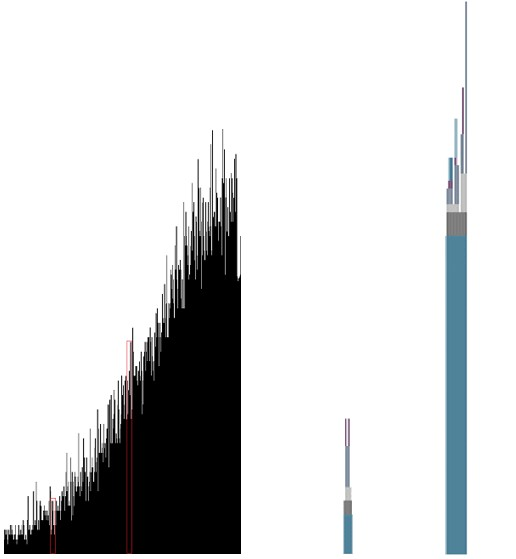
\includegraphics[scale=.45]{sections/images/consciousness_space_subconsciousness.jpg}
	\floatfoot{Menor discrepância das ondas em grandes intervalos.}%\footnotemark}
	\end{figure}
	%\footnotetext{Fonte: note}

Em intervalos menores e com muitos momentos lógicos é observado uma discrepância proporcional maior das amplitudes das ondas. Nesses intervalos podem ser observados sistemas menores de objetos. Quanto menores os intervalos mais desequilibrados eles estarão crescendo sentido a mediana da população, probabilisticamente, conforme Figura \ref{fig:consciousness_space_subconsciousness_min}. Os sistemas de ondas mais complexos e com essa característica podem representar, por exemplo, o átomo que são muito pequenos, se apresentam em enormes quantidades e as partículas que orbitam seu núcleo (elétrons) ficam bem mais distantes dele. Essa maior discrepância está estritamente ligada ao tamanho reduzido destes intervalos, fazendo com que recebam essas novas amostras de uma forma menos uniforme e desequilibrada, o que torna menos precisa o acompanhamento dos seus subintervalos ao seu pico ou a sua linha de referência (a espiral fica mais ampla, alongada e disforme devido a menor uniformidade na sua frequência de correção). As espirais e órbitas podem serem vistas em mais detalhes na subseção da Espiral e órbita.
	\begin{figure}[H]
	\caption{Amplitude de ondas em pequenos intervalos ou comprimentos}
	\label{fig:consciousness_space_subconsciousness_min}
	\centering
	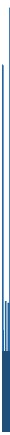
\includegraphics[scale=.45]{sections/images/consciousness_space_subconsciousness_min.jpg}
	\floatfoot{Alta discrepância das ondas em pequenos intervalos.}%\footnotemark}
	\end{figure}
	%\footnotetext{Fonte: note}}

\subsubsubsection{Entrelaçamento}
As amostras que mais se parecem em termos de frequências e distribuição são as amostras que fazem parte da mesma onda. Elas são frequências opostas não sobrepostas que se completam.

Probabilisticamente, as duas partes complementares de uma onda tendem a estar a uma distância aproximadamente iguais, equidistante da mediana, porém essa não é uma regra e as partes complementares de uma onda podem estar em distâncias diferentes em relação à mediana. O fenômeno da paridade das partes de uma onda tem o nome de entrelaçamento de ondas.

Esses pares são formados pela probabilidade de distribuição da população e fazem parte da mesma unidade probabilística. 

Estas unidades probabilísticas formam ondas menores (subconsciências), semelhantes a maior onda do intervalo, comumente entrelaçada pela mediana da população, a consciência. A consciência é a lógica do intervalo, enquanto formam subconsciências ou sub-lógicas, como pequenas ondas de uma onda maior, sendo essas pequenas ondas semelhantes ao padrão da onda maior.
	\begin{figure}[H]
	\caption{Subconsciência}
	\label{fig:consciousness_subconscious}
	\centering
	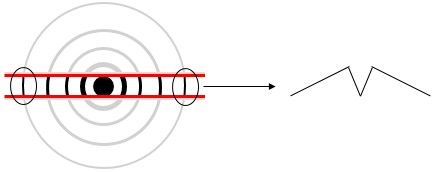
\includegraphics[scale=.8]{sections/images/consciousness_subconscious.jpg}
	\floatfoot{O padrão de ondas forma subconsciências semelhantes ao padrão criado pela consciência, como visto na Figura \ref{fig:trend_chart_of_normal_distribution}.}%\footnotemark}
	\end{figure}
	%\footnotetext{Fonte: note}
	
O entrelaçamento de ondas pode ocorrer em diferentes níveis ou intervalos, conforme visto na Figura \ref{fig:consciousness_subconscious_entanglement}, o que forma sistemas. As chavetas sem bordas (direita) identificam os intervalos os quais uma nova amostra despertou o salto, conforme visto na próxima subseção. Os arcos numerados indicam a ordem dos entrelaçamentos. Um entrelaçamento pode ocorrer de maneira equidistante da mediana não havendo o salto, como o primeiro entrelaçamento (violeta).

O maior entrelaçamento é mostrado nos exemplo da Figura \ref{fig:consciousness_subconscious_entanglement} como o primeiro entrelaçamento (violeta), ocorrido quando esse intervalo era o menor, provavelmente. Os grandes intervalos tendem a ser mantido ordenados pelas reordenações de seus subintervalos subsequentemente. A maior onda é comumente entrelaçada pela mediana da população. 
	\begin{figure}[H]
	\caption{Níveis do entrelaçamento de ondas - comprimentos de ondas}
	\label{fig:consciousness_subconscious_entanglement}
	\centering
	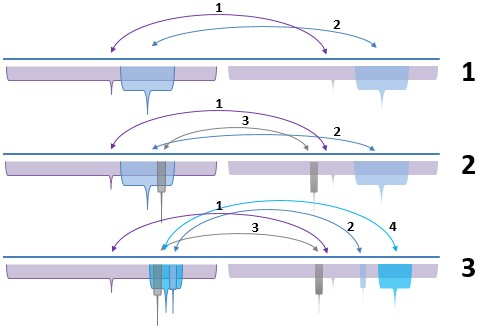
\includegraphics[scale=.8]{sections/images/consciousness_subconscious_entanglement.jpg}
	\floatfoot{Exemplos dos níveis do entrelaçamento de ondas ou níveis dos comprimentos de ondas.}%\footnotemark}
	\end{figure}
	%\footnotetext{Fonte: note}

Se vários intervalos fazem parte de uma mesma discrepância da população, da mesma onda, então estes são subintervalos de um intervalo maior, de uma onda maior.

Os possíveis comprimentos de ondas de uma população são definidos por esses níveis de entrelaçamentos de ondas. Assim, independente da ordem dos saltos, níveis maiores de entrelaçamento são os comprimentos de ondas maiores e níveis menores os comprimentos menores, o que permite que ondas maiores tenham sub-ondas menores. 

Um intervalo superior pode mudar seu par entrelaçado (as demais amostras que não fazem parte de seus subintervalos) sem que afete seus subintervalos, ou seja, cada intervalo ou subintervalo tem seu melhor par correspondente independentemente. Essa é uma condição extraordinária devido as condições de similaridade exigidas para o entrelaçamento. 

Ondas maiores são formados pela adição de suas novas amostras, podendo formar novos subintervalos. O encontro ou separação de dois entrelaçamentos não acarreta um novo entrelaçamento. Assim, ondas maiores também são formados por meio da inclusão (vigor do entrelaçamento) de ondas menores já entrelaçadas quando as áreas dessas ondas estão parcialmente ou totalmente sobrepostas. 

O NADA \underline{NÃO SER} é sinônimo de movimento, de mudança, como apresentado na seção de abertura desse artigo, Lógica. Desta forma, o movimento é assinatura de um intervalo. Essa assinatura corresponde com a distribuição das amostras dentro do intervalo, conforme subseção do Espaço. Os intervalos com assinaturas semelhantes tendem a ter movimentos e velocidades semelhantes, tendem a estar na mesma discrepância de uma onda maior. Essa característica diferencia um intervalo de outro, em outras palavras, discrimina as discrepâncias de uma população.

Os intervalos virtuais são intervalos não entrelaçados, que normalmente formam nuvens virtuais. Essas nuvens virtuais são conjuntos de intervalos virtuais que trocam seus pares entrelaçado constantemente. Esses intervalos virtuais se movem conforme as dimensões espaciais do seu lado do par, melhor visualizado na subseção do Espaço. Um intervalo que perdeu seu entrelaçamento, resultando em um intervalo virtual, continuará sua trajetória até que entrelace novamente, eventualmente com um salto. Os intervalos virtuais podem crescer e estabilizar se tornando um intervalo não virtual.

O vigor de um entrelaçamento é a quantidade de subintervalos que uma onda entrelaçou com outra. O vigor é total quando um subintervalo (que também é uma onda) entrelaçou todos os seus subintervalos dentro da sua onda superior, ou seja, todos os seus subintervalos são frações de seu intervalo superior. O vigor total ocorre mais facilmente quando as ondas de um sistema nascem com o sistema, assim quanto maior o intervalo, maior o número de possíveis subintervalos e maiores as chances de eles se entrelaçarem entre si, devido a distribuição probabilística da população (as amostras são predispostas ainda que aleatórias), o que torna esses intervalos mais e mais estáveis à medida que crescem. Também é possível ter o vigor completo quando um intervalo converge com outro e permanecem assim por um período em que seus subintervalos sofram influência do pico do sistema, a ponto de seus pares entrelaçados estarem dentro da mesma discrepância da população mesmo que não tenham nascido desta mesma discrepância do qual passaram a pertencer. A quantidade de subintervalos que uma onda está constantemente compartilhando com outra onda é o que garante um sincronismo maior ou menor dos movimentos destas ondas, conforme subseção do Espaço. Esse compartilhamento pode ocorrer com os subintervalos já entrelaçados ou com subintervalos não entrelaçados, normalmente parte de uma nuvem virtual. Esse compartilhamento também pode ocorrer em apenas um dos lados do par entrelaçado, como no caso das ondas do mesmo nível.

Como exemplo de vigor parcial, os entrelaçamentos das ondas ou partes maiores de um carro (peças do carro) podem ocorrer com vigor maior ao menor, como a fusão das peças ou solda, colas, algo mais elástico entre outros. Assim, o motor e as rodas de um carro ao acelerar e frear respectivamente, igualmente aceleram e desaceleram suas partes entrelaçadas. Quanto menor o vigor dos entrelaçados, mais as partes sofrem com a inércia, como os objetos e ocupantes soltos no interior de um veículo. Outro exemplo de vigor parcial do entrelaçamento pode ser notado na união molecular.

Como exemplo de vigor total estão os sistemas galácticos, estelares e nucleares, sendo que esse último é menos estável devido ao tamanho reduzido. No entanto, todos esses sistemas têm um nível alto de sincronismo em seus movimentos, melhor explicado na subseção do Espaço.

\subsubsubsection{Salto}
Na Figura \ref{fig:consciousness_space_subconscious_observation_jump} é observado um novo entrelaçamento de intervalos já entrelaçados (representadas por colunas de um histograma para facilitar a visualização do intervalo). Esse novo entrelaçamento ocorre à medida em que as amostras dos pares entrelaçados deixam de ser equivalentes com a adição de novas amostras em um dos lados do par.
	\begin{figure}[H]
	\caption{Novo entrelaçamento}
	\label{fig:consciousness_space_subconscious_observation_jump}
	\centering
	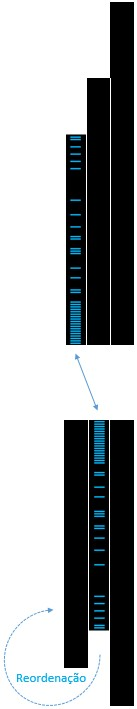
\includegraphics[scale=.53]{sections/images/consciousness_space_subconscious_observation_jump.jpg}
	\floatfoot{Novo entrelaçamento provocado pela não equivalência do par entrelaçado com a adição de novas em um de seus lados.}%\footnotemark}
	\end{figure}
	%\footnotetext{Fonte: note}

O salto ocorre quando um intervalo entrelaça com um intervalo virtual (intervalo não entrelaçado). Neste caso o intervalo entrelaçado surgi em uma região e ao entrelaçar novamente com outro intervalo virtual, surgi em outra.

Como exemplo, um fóton ao entrar no intervalo do elétron pode desequilibrar um dos lados do par entrelaçado do elétron que o faz saltar, porém como o intervalo do elétron é pequeno e o fóton é rápido (por ser ainda menor) ele sai rapidamente do intervalo do elétron que fica desequilibrado novamente e retorna para o nível de energia equivalente ao anterior ao salto.

\subsubsection{Tempo}
O tempo apenas faz sentido quando observado em uma expansão populacional especifica (parcialmente), quando observado em sua integralidade é uma constante transcendente que espelha uma matriz probabilística das infinitas possibilidades. 

\subsubsubsection{Integral}
Na seção inicial Lógica (a seção genitora de todas as demais nesse artigo) foi apresentado que a lógica é uma sequência de negações de si no tempo zero, ou seja, em nenhum momento entre suas negações a lógica passa a \underline{SER}, garantindo a premissa primordial da constante lógica, \underline{NÃO SER}. Quando a expansão é generalizada cada momento lógico está em ordens infinitamente diferentes dentro das infinitas expansões populacionais desta constante, ou seja, a lógica primordial \underline{NÃO SER} é semelhante a uma matriz n x n probabilística quando generalizada, é uma constante transcendente que espelha ou representa essas infinitas possibilidades. Desta forma, a ordem de cada momento lógico só faz sentido na expansão de uma população especifica. Na experiência do tempo conduzida pelo observador a ordenação da sequência é a essência dessa grandeza e, portanto, mais relevante do que sua origem que é de natureza simultânea, o qual transcende o tempo.

\subsubsubsection{Parcial}
O tempo é a adição de novos momento lógicos entre momentos existentes à medida que prossegue a negação de si da lógica. Essas mudanças são acumulativas e a medida que aumentam o número desses momentos lógicos, menos relevante cada novo momento será dentro do intervalo consciente. Um em cem é mais relevante do que um em mil. 
	\begin{figure}[H]
	\caption{Tempo}
	\label{fig:consciousness_time}
	\centering
	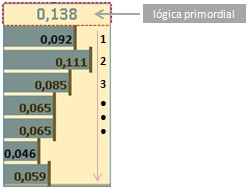
\includegraphics[scale=.8]{sections/images/consciousness_time.jpg}
	\floatfoot{Progressão do tempo conforme os momentos lógicos avançam.}%\footnotemark}
	\end{figure}
	%\footnotetext{Fonte: note}

O tempo também passa em nos intervalos quando estes convergem com outros intervalos e são capazes de interagir com colisões ou entrelaçando seus subintervalos, de acordo com a próxima subsecção do Espaço.

Cada população tem uma ordem diferente em sua sequência e é essa ordem que dá origem à grandeza que chamamos de tempo. É essa ordem do universo ou da consciência que vai dar a noção do que acontece antes ou depois, ou seja, o passado, o presente e as prospecções futuras.

Fluxos temporais de uma população podem ter o mesmo início e até a mesma expansão temporal, infinitamente, a partir da primeira negação da expansão. Desta forma, existem infinitos fluxos temporais na mesma expansão populacional em diferentes pontos dela, conforme expansão em destaque na Figura \ref{fig:consciousness_constant_time}. Logo, não faz sentido associar a quantidade de amostras ou idade do fluxo temporal de um universo particular com a idade da constante lógica \underline{NÃO SER}, a qual precede o tempo. O movimento, mudança ou tempo são versões menores daquilo que é constante e total.
	\begin{figure}[H]
	\caption{Constante lógica - fluxos de tempo da população}
	\label{fig:consciousness_constant_time}
	\centering
	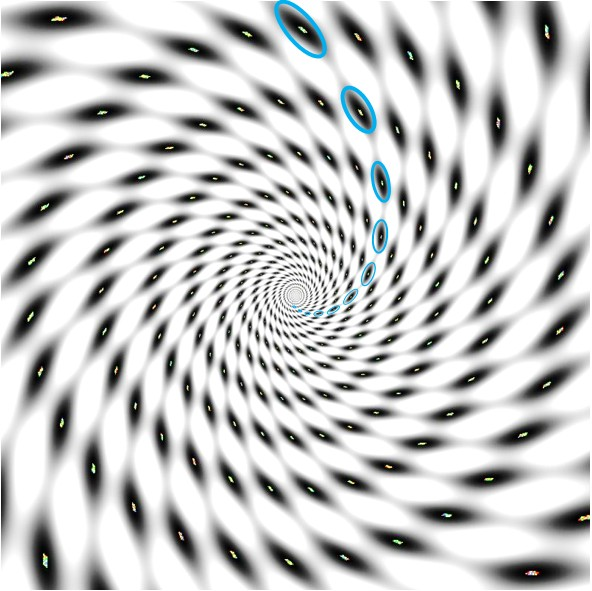
\includegraphics[scale=.6]{sections/images/consciousness_constant_time.jpg}
	\floatfoot{Fonte: Twitter, 2022. \protect\footnotemark}
	\end{figure}
	\footnotetext{\url{https://twitter.com/akiyoshikitaoka/status/851375952051421184}}

Outro fator importante ao observar o tempo (o observador é mais detalhado na subseção da consciência – Observador e a vida) é que, probabilisticamente, subconsciências ou intervalos mais próximos da mediana da população terão uma adição maior de novas amostras em seus intervalos, o que são observados diretamente por essas subconsciências. Por outro lado, subconsciências distantes da mediana da população terão uma adição menor de amostras em seus intervalos e sujeitam-se a um número maior de mudança induzidas indiretamente, conforme detalhado na próxima subseção do Espaço e que também pode ser observado na Figura \ref{fig:consciousness_space_volume_amplitude}. Esse fenômeno de observação temporal proporcionado pela probabilidade de distribuição da população evita o paradoxo dos gêmeos \cite{brasilescola_paradoxo_gemeos}.

Quando a atração gravitacional é mais forte as amostras são mais intensamente distribuídas nesta direção gravitacional, o que, até certo ponto, se opõe a um movimento mais solto em outras direções, ou orbitas. Essa característica talvez influencie no movimento dos relógios atômicos que podem ter um movimento mais uniformes em ambientes com baixa gravidade.

As prospecções de futuro do observador fundamentam-se na probabilidade de distribuição da população e, portanto, da distribuição probabilística de cada subintervalo dela. Logo, o universo tende a ser probabilístico ainda que aleatório em níveis de detalhes, o que faz os eventos serem inusitados ainda que preditos em algum nível, conforme as Figuras \ref{fig:consciousness_logical_moments} e \ref{fig:consciousness}. 

\subsubsection{Espaço}
O tempo e o espaço são provenientes das mesmas amostras da população. O tempo tem relação com a ordem de cada amostra, enquanto o espaço trata da disposição delas na população a cada nova ordem. 

\subsubsubsection{Plano espacial}
O plano espacial é a representação do infinito, do \underline{NÃO SER} em todas as suas possibilidades e do qual emerge os fluxos espaço-temporais como suas possibilidades. Ou seja, é a representação do NADA, do vazio que espelha ou representa todas as possibilidades e está presente em todas as escalas entre qualquer possibilidade espacial e temporal. Esse plano emerge também dentro das escalas do pensamento, onde os exercícios de prospecções (possibilidades futuras) emergem das probabilidades de um intervalo determinado com esse plano ou fluxo lógico das infinitas possibilidades. Logo, ao pensar no NADA naturalmente essa representação lógica do espaço vazio e infinito emerge.

O plano espacial é lógico e plano ainda que suas amostras tendam, probabilisticamente, para a linha de referência da maior onda, que tende a ser separada pela mediana da população.
	\begin{figure}[H]
	\caption{Universo plano}
	\label{fig:consciousness_flat_universe}
	\centering
	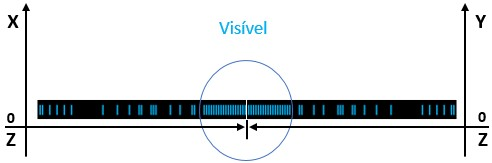
\includegraphics[scale=.6]{sections/images/consciousness_flat_universe.jpg}
	\floatfoot{Concentração de 99\% das amostras.}%\footnotemark}
	\end{figure}
	%\footnotetext{Fonte: note}

\subsubsubsection{Dimensões}
O NADA \underline{NÃO SER} é sinônimo de movimento, de mudança, como apresentado na seção de abertura desse artigo, Lógica. Desta forma, como exibido na Figura \ref{fig:consciousness_flat_universe}, o Z é a representação da quantidade de amostras de uma onda. Logo, o Z é a representação dos entrelaçamentos, que é a única dimensão autêntica e genuína (a essência das dimensões espaciais), sendo o principal sentido do movimento. Como a quantidade de amostras apenas aumentam (o mesmo motivo que faz o tempo fluir apenas em um sentido), os intervalos também se moverão nesse sentido predominante, que neste caso é o de subir. O X e o Y são apenas subdimensões que representam a densidade, o pico, em cada lado do par entrelaçado respectivamente, ou seja, manifestam as diferentes formas de Z subir (quantidade), sendo que X e Y (densidade) podem estar em qualquer lugar (para a esquerda, direita, centralizado entre outras) dentro de cada lado do par entrelaçado. Esses movimentos são mais detalhados na Figura \ref{fig:consciousness_space_plan_nosubinterval}. Posteriormente o X, Y e Z serão tratados como dimensões para facilitar o entendimento.

É mais fácil entender o entrelaçamento quando observado a Figura \ref{fig:consciousness_space_dimensions}. Na parte (A) da Figura, é apresentado como cada lado do par se comporta em suas respectivas dimensões e subdimensões, paralelamente. Fica fácil observar que os intervalos com movimentos semelhantes irão se encontrar e as partes destes intervalos e subintervalos que se corresponderem em cada lado do par se entrelaçam, como a área sobreposta da elipse na parte (B).  
	\begin{figure}[H]
	\caption{Os movimentos dos pares e o encontro - entrelaçamento}
	\label{fig:consciousness_space_dimensions}
	\centering
	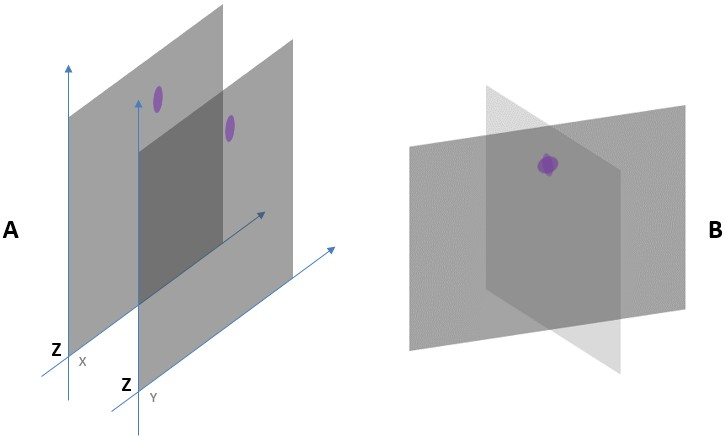
\includegraphics[scale=.7]{sections/images/consciousness_space_dimensions.jpg}
	\floatfoot{Movimentos nas respectivas dimensões e subdimensões de cada lado do par fundamenta o entrelaçamento.}%\footnotemark}
	\end{figure}
	%\footnotetext{Fonte: note}

Quando um ser humano se move, vai de um ponto a outro e retorna (ziguezague), ou qualquer outro movimento, ele está fazendo um movimento semelhante a uma espiral. Observando o movimento como um todo, o ser humano está se movendo também por meio do planeta, sistema solar, galáxia, etc. Não importa as dimensões que o movimento utilizou, probabilisticamente, os movimentos tendem a ser suaves, por abruptos que pareçam localmente (esquerda ou direita, subir ou descer, frente ou atrás). Os movimentos tendem a ser uma variação da espiral, conforme subseção da Espiral e órbita.

\subsubsubsection{Movimento}
Cada nova amostra é tempo e também espaço (movimento e mudança). O movimento é assinatura de um intervalo e essa assinatura corresponde com a distribuição das amostras dentro do intervalo. Um subintervalo, que não contenha subintervalo como na Figura \ref{fig:consciousness_space_plan_nosubinterval}, pode nascer em qualquer lugar. Estes intervalos virtuais se movem conforme as dimensões espaciais do seu lado do par quando não entrelaçados e com as dimensões dos dois lados do par quando entrelaçados. Na Figura \ref{fig:consciousness_space_plan_nosubinterval}, é exibido um intervalo que ainda não contém subintervalos, portanto, sua subida vai ser centralizada se suas amostras são distribuídas uniformemente ou com um pico centralizado, ou será inclinada para a direita ou esquerda à medida que a concentração maior de amostras estiver em um dos lados (é mais comum que a concentração de amostras esteja sentido a mediana da população). No intervalo virtual as dimensões são Z (para subir) e X ou Y, a depender do lado do par, para a densidade de amostras do intervalo não entrelaçado. No intervalo entrelaçado a analogia é a mesma do intervalo virtual, porém as dimensões são Z (para subir em ambos os lados par), X e Y para a densidade de amostras do intervalo em cada lado do par entrelaçado. Um ambiente não rarefeito pode dificultar estes movimentos por conta das colisões. 
	\begin{figure}[H]
	\caption{Intervalo sem subintervalos}
	\label{fig:consciousness_space_plan_nosubinterval}
	\centering
	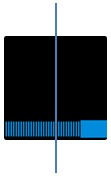
\includegraphics[scale=.7]{sections/images/consciousness_space_plan_nosubinterval.jpg}
	\floatfoot{Movimentação de um intervalo sem subintervalos.}%\footnotemark}
	\end{figure}
	%\footnotetext{Fonte: note}

Teoricamente, a velocidade máxima é de 1 unidade de espaço para 1 unidade de tempo, ou seja, os intervalos se movimentam a uma velocidade menor do que 1 unidade de espaço por 1 unidade de tempo. Não é porque se tem mais amostras que se tem mais velocidade. Se um intervalo tem 2 amostras a direita, por exemplo, ele se moverá a aproximadamente 2 unidades de espaço por 1 unidade de tempo, ou seja, aproximadamente 1 unidade de espaço para cada amostra. Assim, um intervalo tem o limite de velocidade de uma 1 unidade de espaço por amostra por 1 unidade de tempo. O intervalo mais rápido, hipoteticamente, seria o intervalo com uma única amostra totalmente centralizada ou totalmente a direta ou esquerda do intervalo, assim este intervalo atingiria a velocidade máxima, porém sempre existira uma amostra ainda mais centralizada, a direita ou esquerda de um intervalo infinito, conforme as características do intervalo apresentadas na Figura \ref{fig:primordial_logic_representation}. 

A velocidade de um intervalo não está relacionada diretamente com a quantidade de amostras e sim com a proporção da distribuição dessas amostras. Quanto mais desproporcional um intervalo estiver distribuído, quanto mais concentrado for seu pico, mais rápido o intervalo será, independente da direção. Logo, tanto intervalos menores quanto os maiores podem ter grandes velocidades, sendo que os intervalos extremamente grandes tem uma maior facilidade em concentrar o pico, aumento sua desproporção.

Um subintervalo que nasce dentro de seu intervalo superior nasce totalmente sincronizado com esse intervalo superior, ou seja, as amostras dos subintervalos também são amostras do intervalo superior, são amostras compartilhadas, conforme o vigor de seus entrelaçamentos, como visto na subseção do Entrelaçamento. Na Figura \ref{fig:consciousness_space_plan}, a soma dos movimentos dos subintervalos de um intervalo superior movimenta esse intervalo com uma dada direção e velocidade, a qual leva consigo também esses subintervalos menores que são parte sua, ainda que estes subintervalos possam divergir e deixar o intervalo superior em dado momento. Desta maneira, os movimentos das menores ondas foram o movimento da maior onda da população, onde sua direção e velocidade são predominantemente da maioria, normalmente o pico, não obstante o movimento das minorias. E como um bloco, o movimento da maior onda levam as menores, que são partes sua, ainda que algumas destas ondas menores tenham seu próprio movimento e possam escapar em dado momento por divergência em suas direções em relação a direção da maioria.
	\begin{figure}[H]
	\caption{Distribuição espacial e movimento}
	\label{fig:consciousness_space_plan}
	\centering
	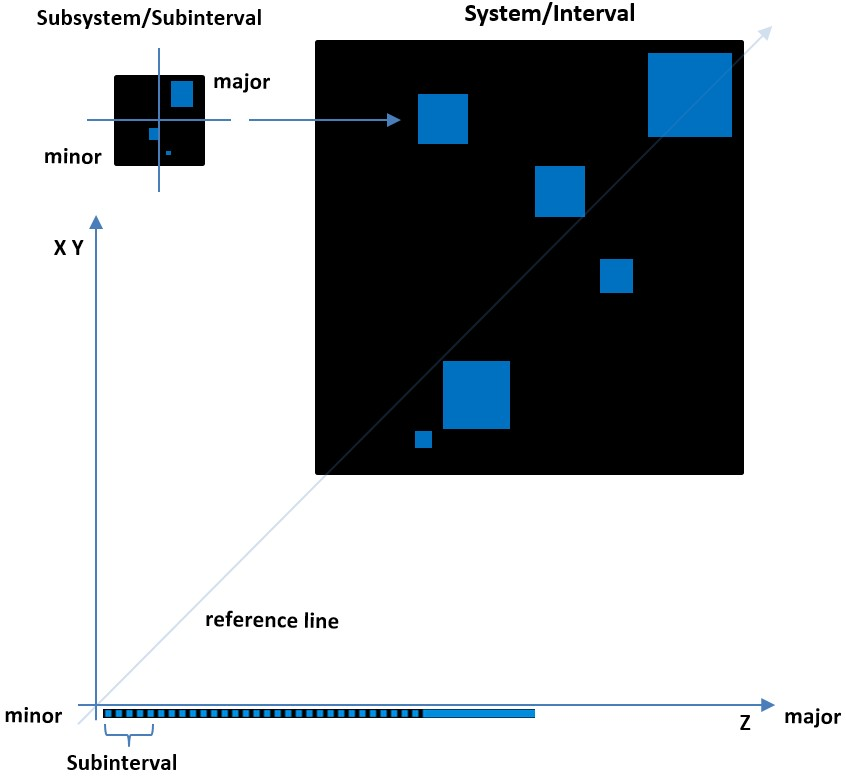
\includegraphics[scale=.6]{sections/images/consciousness_space_plan.jpg}
	\floatfoot{Distribuição espacial e movimento dos subintervalos e do intervalo populacional.}%\footnotemark}
	\end{figure}
	%\footnotetext{Fonte: note}
	
Os intervalos que possuem subintervalos podem se mover em qualquer sentido, uma vez que, seus intervalos que não possuem subintervalos, como na Figura \ref{fig:consciousness_space_plan_nosubinterval}, podem entrelaçar em qualquer lugar e assim esse intervalo pode ter uma distribuição de subintervalos em qualquer sentido, conforme Figura \ref{fig:consciousness_space_plan}. É muito raro a situação em que um intervalo desça (dimensão Z), ainda mais raro quando o intervalo cresce, sendo que está situação tende a ser bem passageira.

O intervalo e seus subintervalos têm suas representações cubica com seus tamanhos referente a quantidade de amostras que eles possuem, eixo Z da Figura \ref{fig:consciousness_space_plan}, a dimensão espacial fundamental e genuína. Uma característica importante com relação ao tamanho dos intervalos e subintervalos pode ser vista na Figura \ref{fig:consciousness_interval_contraction} da subseção do Buraco negro.

Um subintervalo não entrelaçado só influência e é influenciado por um intervalo superior quando está dentro e compartilhando amostras com ele, ou seja, é oriundo da mesma posição populacional da qual se encontra o intervalo superior, ou semelhante quando este tem subintervalos aninhados para compartilhar com o intervalo superior. Da mesma forma e por consequência, um subintervalo entrelaçado só influencia e é influenciado quando dentro do intervalo o qual faz parte, da qual está entrelaçado. Um subintervalo, inclusive virtual, pode estar dentro de um intervalo superior e não compartilhar nenhuma amostra com esse intervalo superior, isso ocorre devido sua distribuição interna de amostras ser completamente diferente do intervalo superior, ou seja, são oriundos de posições diferentes da população e não compartilham a mesma distribuição de amostras.

Como exemplo, é possível imaginar um passageiro dentro de um veículo flutuante no espaço. O movimento do veículo pode arrastar o passageiro, ainda que sofra com uma inércia inicial, que pode ser mínima, até nula, ou desfazer o sincronismo, a depender da intensidade ou vigor dos entrelaçamentos e da aceleração do veículo, podendo até tirar o passageiro do veículo. A inercia do passageiro é menor quanto mais entrelaçado ao veículo ele estiver, como os pés no assoalho, mãos agarradas e sentado em um assento com encosto, por exemplo, conforme o vigor do entrelaçamento explicado na subseção do Entrelaçamento. A velocidade do veículo imposta aos passageiros por meio do entrelaçamento (arraste que é mais forte quanto há aceleração e imperceptível quando estabiliza ou sincroniza) talvez seja um pouco diferente das velocidades dos passageiros que podem estar em ziguezague dentro do veículo, por exemplo, em velocidade distintas entre si e distintas da velocidade do veículo. O movimento do passageiro dentro do veículo também pode influenciar o ângulo e movimento do veículo e se esse movimento não for compatível com o movimento do veículo o passageiro pode deixá-lo. Logo, se os movimentos coincidirem ou variar dentro dos limites dos entrelaçamentos de cada intervalo o sincronismo é mantido. O mesmo acontece com os demais sistemas, ainda mais acentuado, nos subintervalos que nascem dentro do sistema ou estão nele por tempo suficiente, no qual o pico consiga influenciar totalmente na distribuição e densidade das amostras desses subintervalos, refletindo em seus movimentos e velocidades, portanto, refletindo no sincronismo, conforme subseção de Órbitas. A distância não é requisito do entrelaçamento, portanto, não é exclusivo para intervalos próximos.

Na Figura \ref{fig:consciousness_space_matter_antimatter}, nos exemplos A, B e C é exemplificado o movimento dos intervalos de matéria e no exemplo D a antimatéria. Da mesma forma que a matéria comum, os subintervalos de um intervalo de antimatéria também deve ser composto em sua maioria por antimatéria. A antimatéria é detalhada na subseção da Antimatéria. 
	\begin{figure}[H]
	\caption{Movimentação - matéria e antimatéria}
	\label{fig:consciousness_space_matter_antimatter}
	\centering
	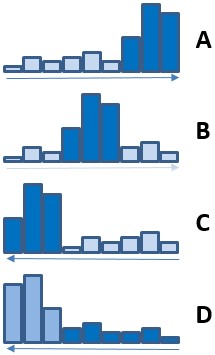
\includegraphics[scale=.7]{sections/images/consciousness_space_matter_antimatter.jpg}
	\floatfoot{Movimentos de matéria e antimatéria.}%\footnotemark}
	\end{figure}
	%\footnotetext{Fonte: note}

No exemplo A, da Figura \ref{fig:consciousness_space_matter_antimatter}, o pico do intervalo está a sua direita, o que provoca uma velocidade maior sentido a mediana da população. No exemplo B, o pico está centralizado no intervalo, contudo suas amostras estão mais concentradas levemente sentido a mediana da população, o que provoca uma velocidade menor neste sentido e a depender do ponto de vista do observador esse intervalo pode parecer estar indo para trás. No exemplo C, pico do intervalo está a sua esquerda, o que provoca uma velocidade maior ao contrário da mediana da população e é mais comum em pequenos intervalos, no entanto, os subintervalos em azul escuro (o pico), por terem mais amostras, tendem a ter mais facilmente suas amostras sentido a mediana e poderão andar para frente mais rápidos que os demais subintervalos estabilizando o intervalo com o pico ao centro ou mais à direita. O exemplo D é parecido com o C, porém crescimento dos subintervalos deste exemplo estão claramente no sentido contrário da mediana da população representando a antimatéria.
	
Na Figura \ref{fig:consciousness_space_waves}, é exibido um exemplo da densidade de amostras de uma população, onde os pares que tendem a mesma distribuição probabilística são colocados lado a lodo e representados em forma de histograma. A formação desses pares é proveniente do entrelaçamento de ondas.
	\begin{figure}[H]
	\caption{Pares entrelaçados representados em três dimensões espaciais}
	\label{fig:consciousness_space_waves}
	\centering
	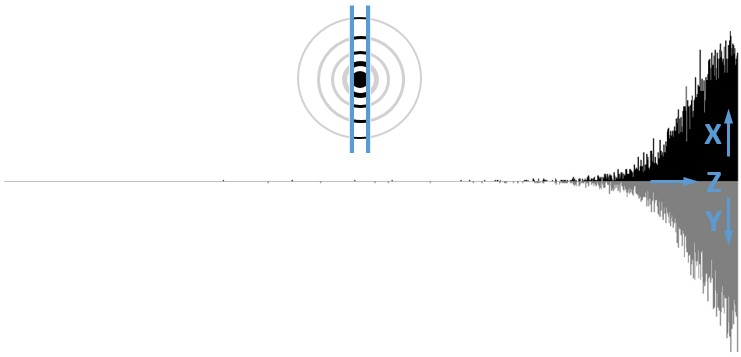
\includegraphics[scale=.7]{sections/images/consciousness_space_waves.jpg}
	\floatfoot{Exemplo de ondas entrelaçadas, representadas em forma de histograma e obtidas pelo algoritmo Logic\_WavePattern. \footnotemark}
	\end{figure}
	\footnotetext{O algoritmo Logic\_WavePattern pode ser visto no Apêndice \ref{app:algoritmos}.}

Ao representar as grandezas espaciais do gráfico da Figura \ref{fig:consciousness_space_waves} em um gráfico de distribuição 3D e distribuir seus pontos de extremidade (desprezando seus volumes e possíveis pontos internos), obtém-se algo parecido com uma espiral (como redemoinhos no ar ou na água) mesmo em volumes muito pequenos de dados (poucos momentos lógicos), conforme Figuras \ref{fig:consciousness_space_3DScatter15000-10} e \ref{fig:consciousness_space_3DScatter_200000-2}. Os pontos tendem a se moverem em forma de espiral, aproximadamente, conforme mostra a subseção posterior. 
	\begin{figure}[H]
	\centering
		\begin{subfigure}[H]{0.47\linewidth}
		\centering
		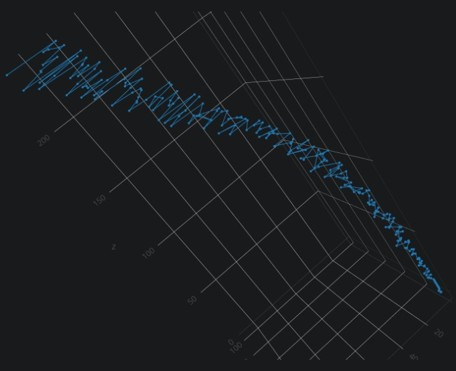
\includegraphics[width=1\linewidth]{sections/images/consciousness_space_3DScatter15000-10.jpg}
		\caption{15.000 amostras ou momentos}
		\label{fig:consciousness_space_3DScatter15000-10}
		\end{subfigure}
	
		\begin{subfigure}[H]{0.47\linewidth}
		\centering
		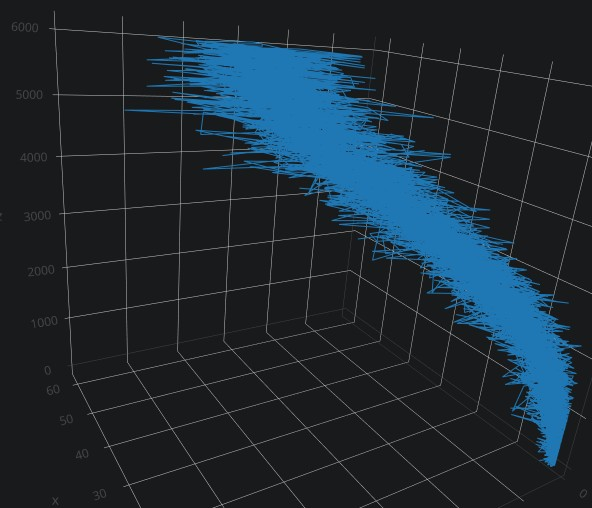
\includegraphics[width=1\linewidth]{sections/images/consciousness_space_3DScatter_200000-2.jpg}
		\caption{200.000 amostras ou momentos}
		\label{fig:consciousness_space_3DScatter_200000-2}
		\end{subfigure}%
	\caption{Gráficos de dispersão 3D gerados com pontos semelhantes aos da Figura \ref{fig:consciousness_space_waves}}
	\floatfoot{O histograma no padrão de ondas e os dados para gerar os gráficos de dispersão 3D podem ser obtidos com a execução do algoritimo Logic\_WavePattern. \protect\footnotemark}
	\end{figure}
	\footnotetext{O algoritmo Logic\_WavePattern pode ser visto no Apêndice \ref{app:algoritmos} e os gráficos de dispersão 3D podem ser acessados em: \url{https://chart-studio.plot.ly/create/?fid=ren.stuchi:5&fid=ren.stuchi:4} e \url{https://chart-studio.plot.ly/create/?fid=ren.stuchi:7&fid=ren.stuchi:6}}

\subsubsection{Forças fundamentais}
A força gravitacional, a força eletromagnética e a força nuclear correspondem às chamadas forças fundamentais da natureza. Essas forças fundamentais não são forças propriamente, mas sim aspectos probabilísticos de distribuição da população e do entrelaçamento de ondas.

\subsubsubsection{Força gravitacional}
A força gravitacional não é uma força propriamente e sim um aspecto da probabilidade de distribuição de novas amostras sentido a mediana da população, conforme teorema central do limite. Esse sentido probabilístico faz com que as ondas tenham um caminho provável a seguir dentro da população, ou seja, o pico de amostras da população ou o pico da maior onda da população. Da mesma maneira, fazem também com que as amostras dentro de um intervalo tenham um caminho provável a seguir, o pico de amostras do intervalo ou o pico da onda. Estes picos de amostras costumam ser a parte mais facilmente observáveis no intervalo de amostras desde que ocupem uma área não tão pequena.

Na Figura \ref{fig:consciousness_gravitational_force} pode ser visto que a parte mais facilmente observável está levemente a direita no pico da onda. Essa onda tende a caminhar para cima e para a direita, em uma diagonal sentido ao pico do seu intervalo superior. 
	\begin{figure}[H]
	\caption{Força gravitacional}
	\label{fig:consciousness_gravitational_force}
	\centering
	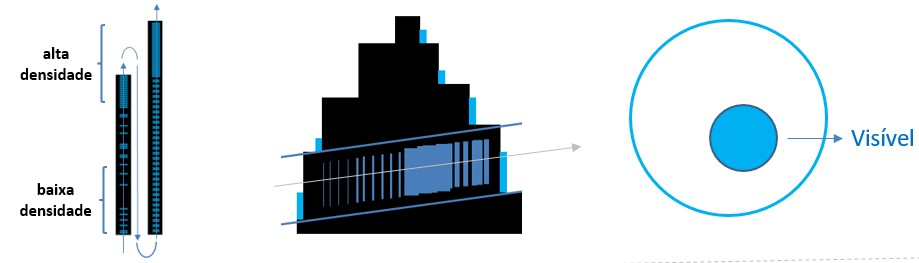
\includegraphics[scale=.7]{sections/images/consciousness_gravitational_force.jpg}
	\floatfoot{Aspecto gravitacional, o sentido probabilístico da distribuição de novas amostras dentro de um intervalo.}%\footnotemark}
	\end{figure}
	%\footnotetext{Fonte: note}

A área de um intervalo cresce de forma quadrática, uma vez que o salto provocado pelo entrelaçamento de ondas e a própria distribuição probabilística das amostras tendem a manter um crescimento equivalente nos pares que formam a onda. Esse aspecto configura a lei do inverso do quadrado, onde, no caso da gravidade, quando mais perto os objetos, maiores serão as chances probabilísticas das novas amostras do objeto menor ir em direção ao objeto maior (o pico da onda), que por estar dentro de uma área quadrada menor e por consequência de menor possibilidades de posicionamento das amostras, as chances desses objetos se aproximarem com uma quantidade bem menor de momentos lógicos aumenta muito. Assim, quanto mais longe os objetos, maior a área, maior as possibilidades de posicionamento e mais momentos lógicos são precisos para a aproximação, caracterizando assim uma atração menor. A probabilidade também pode afastar objetos mais rarefeitos que devem estar mais afastados da parte mais facilmente observável e densa de amostras, como no caso do gás hélio, por exemplo. A distribuição de novas amostras nos intervalos rarefeito são mais lentas (caso contrário não seriam rarefeito) do que nas partículas mais densas que tomam a frete dessas partículas menos densas afastando-as do pico da onda. 

\subsubsubsection{Força eletromagnética}
A força eletromagnética não é uma força propriamente e sim um aspecto do entrelaçamento de ondas que se intensifica em intervalos ou comprimentos de ondas com baixa entropia e com a aproximação espacial (redução de diferenças nos eixos X, Y e Z) desses intervalos.

Quando os intervalos têm baixa entropia, a sobreposição total ou parcial de suas áreas facilita a reordenação de seus pares entrelaçados, e um exemplo disso pode ser a sobreposição da área do elétron com as nuvens fotônicas de outros elétrons ou átomos. Essa reordenação é uma tentativa de equalizar essas ondas em uma onda única de baixa entropia, o que também tornando viável a troca de muitos desses pares pelos da nuvem virtual não entrelaçada (nuvem virtual de amostras não entrelaçadas, normalmente ao redor do pico do intervalo ou subintervalos, conforme subseção do Entrelaçamento), podendo resultar na aproximação dessas ondas devido a essa reordenação.

As linhas azuis da Figura \ref{fig:consciousness_electromaagnetic_force} mostra onde é mais frequente a troca dos pares de ondas pelo entrelaçamento de ondas, ou seja, onde se tem a maior probabilidade das ondas serem parecidas. Por isso os imãs tentam se virar para se conectar quando estão face a face com o mesmo polo. A linha cinza mostra as conexões que ocorrem em número bem menor.
	\begin{figure}[H]
	\caption{Força eletromagnética}
	\label{fig:consciousness_electromaagnetic_force}
	\centering
	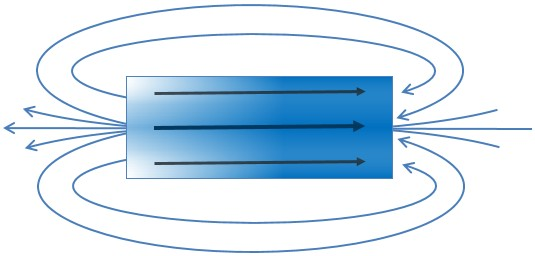
\includegraphics[scale=.7]{sections/images/consciousness_electromaagnetic_force.jpg}
	\floatfoot{Aumento das possibilidades de entrelaçamento de ondas devida a equalização probabilística em objetos próximos e de baixa entropia.}%\footnotemark}
	\end{figure}
	%\footnotetext{Fonte: note}

A Figura \ref{fig:consciousness_electromaagnetic_force_entropy} mostra um exemplo de baixa entropia. 
	\begin{figure}[H]
	\caption{Força eletromagnética - entropia}
	\label{fig:consciousness_electromaagnetic_force_entropy}
	\centering
	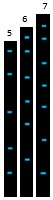
\includegraphics[scale=.9]{sections/images/consciousness_electromaagnetic_force_entropy.jpg}
	\floatfoot{Aumento das possibilidades de entrelaçamento de ondas devido à baixa entropia.}%\footnotemark}
	\end{figure}
	%\footnotetext{Fonte: note}

O aspecto eletromagnético está intimamente relacionado com a baixa entropia de um intervalo e a possibilidade de entrelaçamento de seus pares com os pares ao redor. A baixa entropia de um intervalo indica que suas amostras estão em uma ordem qualquer em seu interior.

Probabilisticamente, os pares de ondas mais parecidos estão nas regiões mais próximas (linhas azuis do Figura \ref{fig:consciousness_electromaagnetic_force}). Isso ocorre devido ao crescimento do número de amostras sentido a mediana da população, porém não é regra e os polos podem se inverter, ou seja, ter mais ligações com a região de menor probabilidade, ainda que a maior parte dos pares que compõem essa região estejam de forma crescente sentido a mediana.

\subsubsubsection{Força nuclear}
Os mesmos aspectos probabilísticos que regem a gravidade e que podem ser vistos na Figura \ref{fig:consciousness_gravitational_force} também regem as chamadas forças nucleares. A diferença é que nas forças nucleares os intervalos são menores possibilitando uma quantidade muito maior de saltos e suas ondas são mais discrepantes, conforme mostra a Figura \ref{fig:consciousness_space_subconsciousness_min}.

As forças nucleares forte e fraca representam grandes concentrações de momentos lógicos por intervalo populacional, uma alta densidade em um pequeno intervalo. A grande concentração dessas amostras está no pico do intervalo, que ocupa um subintervalo cada vez menor dentro da onda (proporcionalmente), devido à alta concentração de amostras em intervalos cada vez menores, conforme Figura \ref{fig:total_comparison_chart_with_99_range}.

É importante destacar em relação aos movimentos dos elétrons e núcleo atômico, como visto na subseção de Órbitas, que o núcleo atômico está em movimento tão rápido no espaço assim como todos as suas ondas superiores. Os sistemas estelares estão na mesma velocidade que suas galáxias entre outros, devido ao vigor do entrelaçamento das ondas em todos os níveis de entrelaçamento, conforme subseção do Entrelaçamento, tornando o movimento síncrono em grande medida. Os núcleos, sejam eles estelares, atômicos ou qualquer outro tendem a estar mais rápidos no espaço e puxam suas orbitas, mostrado na subseção de Órbitas. Esse movimento sincronizado e rápido em uma direção do espaço não provoca repulsão.

O núcleo é um subintervalo do intervalo atômico, é o pico onda. Os elétrons também são subintervalos do intervalo atômico, apesar da alta discrepância entre o núcleo atômico e seus elétrons. Essa discrepância é comum em pequenos intervalos como o atômico, conforme a Figura \ref{fig:consciousness_space_subconsciousness_min}, o que tende a acentuar ainda mais a discrepância do pico com o restante da onda. Entretanto, nos subintervalos do pico ou núcleo essa discrepância é menor devido a estes serem bem mais densos que os elétrons e estarem dentro da mesma probabilidade de distribuição, os 99\% das amostras do intervalo, aproximadamente. Outro fator que faz a discrepância dos subintervalos do pico diminuir ainda mais é a abundância destes subintervalos, assim eles tendem a trocar subintervalos com outros núcleos atômicos e afinar ainda mais suas distribuições de amostras (movimento e velocidade, conforme as elipses correspondes da Figura \ref{fig:consciousness_space_dimensions}). Por estarem próximos e com essa correspondência maior, aumenta as chances que compartilhem mais subintervalos aninhados entre si, aumentando o vigor entre estes subintervalos do mesmo núcleo, o que aumenta a correspondência dos movimentos entre eles facilitando a aproximação. Desta forma, fica fácil perceber que mesmo em intervalos com vigor total (onde todos os subintervalos entrelaçados estão dentro do seu intervalo superior) seus subintervalos são mais ou menos separáveis a medida que estão mais ou menos entrelaçados entre si (quando o entrelaçamento ocorre em apenas um lado do par por estarem no mesmo nível, conforme subseção do Entrelaçamento).

Outro fator importante é que em intervalos menores de amostras, como os subintervalos aninhados do núcleo atômico, pode ser mais comum que estes se comportem como ondas ou nuvens mais ou menos densas, sem um pico definido e visível, devido a tendência que suas discrepâncias sejam maiores à medida que os subintervalos diminuem.

A penetração desses intervalos pequenos e densos por uma quantidade excessiva de momentos lógicos (outro intervalo semelhante), em um curto período, faz com que os inúmeros pares de seus subintervalos oscilem potencializando os saltos. Dessa forma os subintervalos saltam de forma continua, progressiva e rapidamente até que a probabilidade de distribuição da população normalize todo o intervalo posteriormente. Junto dos saltos que irão provocar movimentos em grande número de partículas ou intervalos ao redor, há um enorme número de atritos em velocidades tremendas provocados pelas colisões dessas pequenas partículas ou nuvens que provocam grandes ondas de choque.

Uma vez que os subintervalos do núcleo atômico estão muito próximo e afinados em seus movimentos e velocidades, suas entropias tendem a ser menores. Portanto, na aproximação de dois picos com baixa entropia tende a ocorrer o mesmo efeito encontrado quando tentado aproximar dois imas por meio do mesmo polo, conforme explicado na Figura \ref{fig:consciousness_electromaagnetic_force}. 

\subsubsection{Espiral e órbita}
Como as coordenadas X, Y e Z dos pares emaranhados de uma população tendem a aumentar, a disposição dessas em um sistema tridimensional de coordenadas vai seguir uma referência diagonal entre esses três eixos, conforme Figura \ref{fig:consciousness_space_spiral_reference_line}. O padrão de espiral observado não invalida outros possíveis movimentos no espaço. Muitas vezes não é possível observar o padrão de espiral imediatamente nos movimentos de um intervalo (subintervalo), porém esse padrão está por traz de muitos destes movimentos. Ao pegar os movimentos humanos, como exemplo, tem-se os ciclos predominantes de ir e voltar para casa, ir e voltar ao trabalho, acordar e dormir, ou seja, os hábitos se assemelham a movimentos em ciclos, movimentos espirais.
	\begin{figure}[H]
	\caption{Sistema tridimensional de coordenadas}
	\label{fig:consciousness_space_spiral_reference_line}
	\centering
	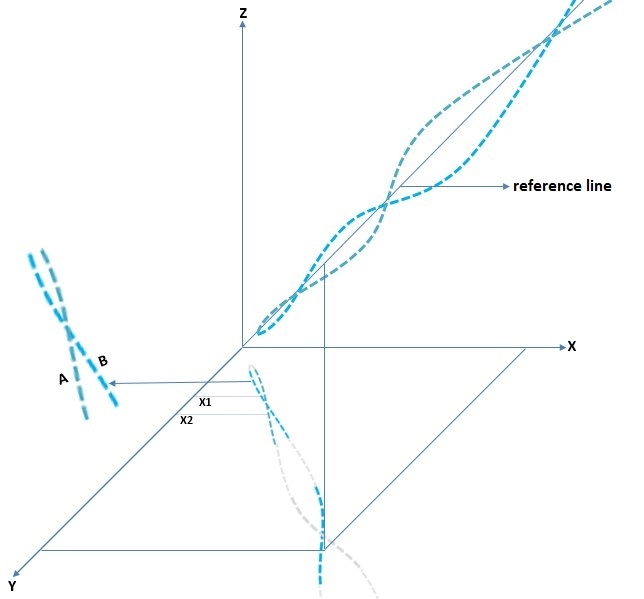
\includegraphics[scale=.7]{sections/images/consciousness_space_spiral_reference_line.jpg}
	\floatfoot{Linha de referência probabilística para distribuição de uma população em um plano tridimensional.}%\footnotemark}
	\end{figure}
	%\footnotetext{Fonte: note}}

Na Figura \ref{fig:consciousness_space_spiral_reference_line} também podem ser observado os pontos X1 e X2. Esses pontos foram espelhados nas coordenadas X e Y para facilitar a observação de que mesmo na parte inferior da espiral o intervalo continua a somar amostras, ainda que em menor quantidade do que quanto subindo para a parte superior da espiral. A linhas tracejadas mostram os caminhos mais prováveis para os intervalos A e B. Dessa forma, quando uma parte do intervalo está em seu ponto médio máximo (eixos X e/ou Y) a tendência probabilística é que ele receba menos amostras do que a parte do intervalo que está em seu ponto médio mínimo. Esse efeito espiral é mais notável quanto maior for um intervalo e sua quantidade de amostras, pois mais prováveis e estáveis serão esses caminhos.

O movimento contínuo num ambiente rarefeito também ajuda na formação e manutenção das espirais. À medida que as amostras são adicionadas aos subintervalos, as suas velocidades tendem a aumentam em direção à linha de referência, e como esta adição não é uniforme (variando entre picos e vales) e o movimento é aproximadamente contínuo, os subintervalos podem derivar ou deslizar de um lado da linha de referência para o outro.

Cada intervalo ou subintervalo (comprimento de ondas) tem sua própria linha de referência. Assim como dentro de um metro existem os centímetros, milímetros etc., dentro de um intervalo e subintervalos podem existir inúmeros outros, conforme exibido abaixo.
	\begin{figure}[H]
	\caption{Intervalos e linhas de referências}
	\label{fig:consciousness_space_spiral_underlines}
	\centering
	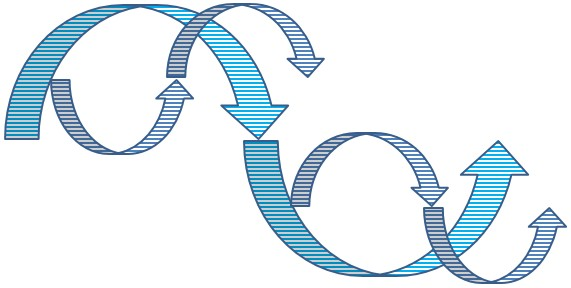
\includegraphics[scale=.5]{sections/images/consciousness_space_spiral_underlines.jpg}
	\floatfoot{Espirais em diferentes intervalos e suas linhas de referências.}%\footnotemark}
	\end{figure}
	%\footnotetext{Fonte: note}}

\subsubsubsection{Órbitas}
Órbita pode ser definida nesse estudo como o conceito das espirais somada a orientação de um pico probabilístico (gravidade) ao invés da linha de referência das espirais, apenas.

Os sistemas que orbitam como descrito anteriormente (em espiral - orientada pela linha de referência) são sistemas ou intervalos em que seu pico está subdividido em subintervalos e não formam um centro de gravidade, ou seja, todos os subintervalos do pico não estão concentrados em um ponto do sistema, orbitando dessa forma a linha de referência do intervalo. Provavelmente os aglomerados de galáxia, e os superaglomerados sejam exemplos dessa orbita. A orbita espiral (orientada pela linha de referência) não está restrita a sistemas grandes, essa orbita é uma característica que pode acontecer em qualquer tamanho de intervalo.

Outro tipo de órbita é definido quando os subintervalos que orbitam o pico da onda (que representa aproximadamente 99,9\% das amostras do intervalo) diminuem sua velocidade de orbita à medida que se afastam do pico. Na Figura \ref{fig:consciousness_elliptical_orbit_system} as colunas do histograma em azul representam o pico da onda. Essa diminuição de velocidade ocorre gradualmente a medida que esses intervalos em cinza se afastam do pico da onda, recebendo assim uma quantidade menor de amostras, diminuindo sua aceleração. O sistema solar é possivelmente um exemplo desse tipo de órbita. As órbitas atômicas também podem se assemelhar a esse tipo de órbita devido as diferenças de energias entre as camadas estruturadas pelos saltos.  
	\begin{figure}[H]
	\caption{Órbitas dos subintervalos fora do pico da onda}
	\label{fig:consciousness_elliptical_orbit_system}
	\centering
	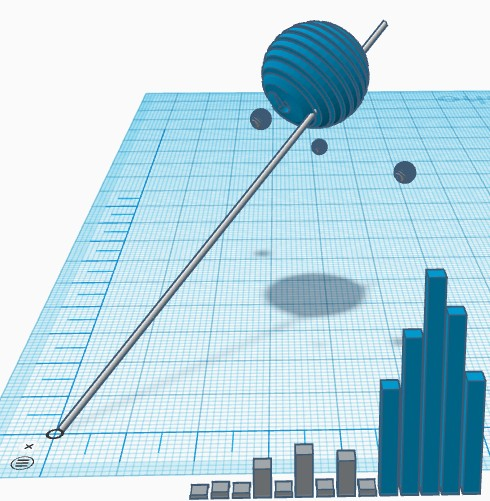
\includegraphics[scale=.7]{sections/images/consciousness_elliptical_orbit_system.jpg}
	\floatfoot{Os subintervalos diminuem de velocidade conforme se afastam do pico da onda.}%\footnotemark}
	\end{figure}
	%\footnotetext{Fonte: note}

Ainda outro tipo de órbita é definido quando os subintervalos que orbitam o pico da onda mantêm uma velocidade média constante, independente da distância do pico. Isso ocorre porque esses subintervalos também fazem parte do pico da onda em azul, conforme Figura \ref{fig:consciousness_circular_orbit_system}. Assim, por estes subintervalos permanecerem em órbita dentro do subintervalo de 99,9\% da onda, suas velocidades não diminuem. Esses 99,9\% da onda é parte mais facilmente visível, portanto, a parte observada das galáxias, provavelmente. Talvez essa característica também seja responsável pelos anéis dos planetas. 
	\begin{figure}[H]
	\caption{Órbitas dos subintervalos dentro do pico da onda}
	\label{fig:consciousness_circular_orbit_system}
	\centering
	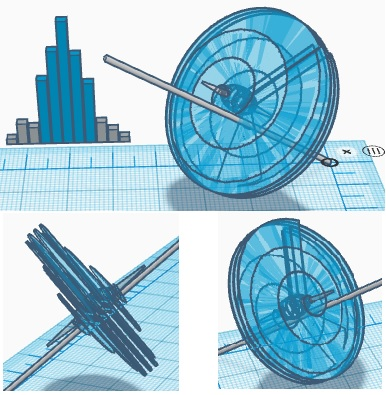
\includegraphics[scale=.9]{sections/images/consciousness_circular_orbit_system.jpg}
	\floatfoot{Os subintervalos mantêm a velocidade conforme se afastam do pico da onda.}%\footnotemark}
	\end{figure}
	%\footnotetext{Fonte: note}

Para a distância dos subintervalos em órbita a gravidade exerce mais uma orientação do que uma atração. Porém como o movimento é praticamente continuo em ambientes rarefeitos e essa orientação é permanente, as órbitas vão se formando e sendo mantidas pela velocidade crescente desses subintervalos, que tende a afastá-los. 

Conforme afirmado na subseção do espaço, uma nova amostra em um subintervalo o move e seus intervalos superiores. Também novas amostras no intervalo superior movem os intervalos inferiores, pois são frações da mesma onda. Desta forma, uma onda inferior permanecerá na onda superior quando sua velocidade for menor que a velocidade de pico da onda superior e sua trajetória não for oposta à trajetória da onda superior. O movimento da onda superior arrasta seus subintervalos, que com velocidades probabilísticas mais baixas continuarão a se mover dentro de sua onda superior, pois mesmo com velocidades mais baixas são arrastados pelo movimento da onda superior, que também é composta pelo movimento de seus subintervalos.

Dobrar a quantidade de amostras de um intervalo não irá dobrar definitivamente a velocidade de um intervalo, pois se tem o dobro de amostras para mover tornando inalterada a velocidade. Porém, probabilisticamente, quanto maior a quantidade de amostras de uma onda, mais essas amostras estarão sentido à mediana da população e menos relevantes se tornam as amostras contrárias, o que torna a velocidade probabilística dos picos de ondas superiores à velocidade de seus subintervalos. Isso não é uma regra e um subintervalo pode ter velocidade superior ao pico de sua onda superior ou seu movimento pode ser contrário ao movimento do pico da onda superior, fazendo com que ele saia naturalmente da gravitação de sua onda superior (e isso ocorre mais facilmente com intervalos bem pequenos e rápidos favorecido por seu movimento num ambiente rarefeito devido ao tamanho). 

\subsubsubsection{Matéria escura e energia escura}
Os intervalos naturalmente se afastam com velocidades crescentes por receberem mais amostras em direção à linha de referência ou pico da onda de seus intervalos superiores e por se moverem em um ambiente rarefeito.

As espirais podem ocorrer sem a necessidade de um pico de onda concentrado, mas quando há tal concentração no pico da onda, as órbitas podem ocorrer dentro ou fora dos 99,9\% das amostras do pico, resultando em órbitas que mantêm suas velocidades médias constantes quando longe do pico (dentro dos 99,9\%) ou órbitas que diminuem suas velocidades quando estão longe do pico (fora dos 99,9\%).

Portanto, matéria escura e energia escura não são matéria nem energia, mas aspectos probabilísticos da distribuição de amostras em uma população que se assemelha à distribuição normal.

\subsubsection{Antimatéria}
Quando um intervalo tende a concentrar suas amostras sentido da mediana, o que é o sentido provável conforme teorema central do limite, dá-se o nome de matéria. A antimatéria é o contrário, quando um intervalo tende a concentrar suas amostras no sentido oposto à mediana. 

A maneira mais simples de visualizar o sentido probabilístico das amostras de qualquer comprimento de onda é observar a \textbf{linha de referência probabilística}, conforme exibido na Figura \ref{fig:consciousness_space_spiral_reference_line}. Quanto maior a quantidade de amostra de um intervalo maior será sua tendência probabilística sentido a mediana da população.

Na Figura \ref{fig:consciousness_concentration_of_opposite_samples} é exibido dois intervalos idênticos com suas amostras em concentrações opostas.
	\begin{figure}[H]
	\caption{Parte de um intervalo idêntico com suas concentrações de amostras opostas}
	\label{fig:consciousness_concentration_of_opposite_samples}
	\centering
	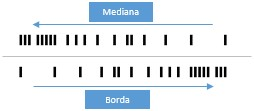
\includegraphics[scale=1.2]{sections/images/consciousness_concentration_of_opposite_samples.jpg}
	\floatfoot{Parte de um intervalo idêntico distribuídos de formas opostas.}%\footnotemark}
	\end{figure}
	%\footnotetext{Fonte: note}

O merge ou soma dos intervalos opostos da Figura \ref{fig:consciousness_concentration_of_opposite_samples} os tornaria um intervalo simétrico, ou seja, não estaria em nenhum dos sentidos.
Na Figura \ref{fig:consciousness_concentration_of_opposite_samples_within_range} é exibido uma população com suas concentrações de amostras sentido à mediana e outra com suas concentrações sentido às bordas do intervalo.
	\begin{figure}[H]
	\caption{Populações com suas concentrações de amostras opostas}
	\label{fig:consciousness_concentration_of_opposite_samples_within_range}
	\centering
	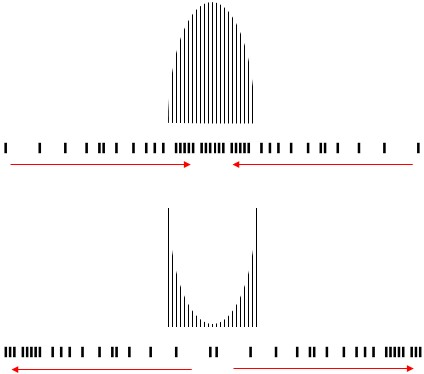
\includegraphics[scale=.7]{sections/images/consciousness_concentration_of_opposite_samples_within_range.jpg}
	\floatfoot{Populações distribuídas em sentidos contrários.}%\footnotemark}
	\end{figure}
	%\footnotetext{Fonte: note}

\subsubsection{Buraco negro}
A área de um intervalo cresce à medida que novas amostras são adicionadas na população, conforme Figura \ref{fig:consciousness_space_volume_amplitude}, e com a soma de outros intervalos já entrelaçados, como mostra o subintervalo superior direito na Figura \ref{fig:consciousness_interval_contraction}. Contudo, os intervalos que recebem uma grande quantidade de amostras dentro da população tendem a formar cada vez mais subintervalos a diferentes níveis, que contraem a área ocupada destes intervalos (devido ao entrelaçamento de ondas do subintervalos menores sustentar essas áreas aproximadamente quadráticas), como mostra os subintervalos roxos e azuis na Figura \ref{fig:consciousness_interval_contraction}. Assim, essa relação do tamanho do intervalo com sua quantidade de amostras e os seus subintervalos é o aspecto que pode ajudar a descrever os chamados buracos negros, onde o pico da onda irá ocupar um subintervalo proporcional cada vez menor dentro do intervalo da onda, mesmo com uma concentração de amostras crescentes. Esses picos são frequentemente encontrados do meio para frente de um intervalo ou sistema (o núcleo ou pico do sistema).
	\begin{figure}[H]
	\caption{Contração do intervalo}
	\label{fig:consciousness_interval_contraction}
	\centering
	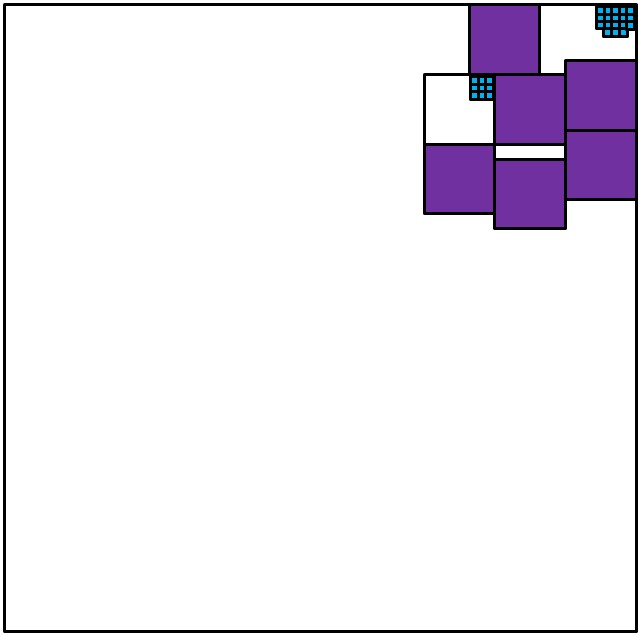
\includegraphics[scale=.5]{sections/images/consciousness_interval_contraction.jpg}
	\floatfoot{Relação do tamanho do intervalo e sua possível contração à medida que surgem novos subintervalos.}%\footnotemark}
	\end{figure}
	%\footnotetext{Fonte: note}
	
\subsubsection{Observador e a vida}
Os intervalos de ondas (comprimentos de ondas) que uma subconsciência (sub-lógica) é capaz de observar depende do comprimento de ondas que a própria subconsciência é constituída. Dentre todas as possibilidades de intervalos ou comprimento de ondas permitidos por uma população, o observador está em um deles.

A capacidade de comparar ou distinguir a ordem das mudanças de uma sequência amostral é a capacidade lógica de um observador, o observador do tempo (passado e presente). A velocidade dessa observação é dada pelo range que o observador é capaz de comparar, ou seja, o qual rápido ele for capaz de distinguir pequenas mudanças (poucas amostras) o fará perceber que mudanças maiores levam mais tempo (muitas amostras). 

A capacidade lógica de fazer prospecções probabilísticas, dentro das limitações lógicas do observador e com base na probabilidade da distribuição do intervalo ou subintervalo observado é a essência do pensamento e, portanto, da vida. Essas prospecções estão fundamentadas na probabilidade de distribuição de cada intervalo (no sentido do intervalo) e, portanto, estão relacionadas com a detecção de padrão e com possibilidades probabilísticas futuras.

A capacidade de comparar ou distinguir ondas lógicas, subconjuntos ou subconsciências, é a capacidade que define o sujeito (eu). A razoabilidade dessa definição depende da proporcionalidade dessa capacidade de comparação.

Comumente, as formas mais notáveis de vida se multiplica por estarem na média probabilística do intervalo entre seus picos e vales, por mais diferente que sejam. Porém, algo muito discrepante ou diferente do padrão médio do intervalo tende a não multiplicar e permanecer.

A vida \underline{NÃO É}, como qualquer outra lógica. E seu sentido está no que a lógica é em sua essencial. A lógica em sua essência probabilística é a ordem que emerge do caos das infinitas possibilidades, é o que a física chama de gravidade e a Bíblia de Amor quando diz que Deus é Amor. Logo, o sentido da vida é ser diferença, que em contraponto a uma linha reta (representando a nulidade, indiferença ou inexistência) se faz discrepante com seus picos (ondas), picos estes que entrelaçam e compartilham seus subintervalos com os demais de suas ondas, tornando seus movimentos e de seus subintervalos mais harmônicos e sincronizados, o que em algumas escalas são chamadas de orbitas em outras de amor, quando o ser humano orbita aquilo que ama, seja o que for. Esse é o sentido da vida e de todo o universo, e não apenas isso, além de dar o sentido é o que os tornam possíveis. O ser humano talvez possa ser considerado o pico da onda dos subsistemas considerados vivos na terra, tendo a capacidade de dominar e cuidar dos demais. 

O livre arbítrio está na aleatoriedade das novas amostras, apesar do sentido probabilístico destas amostras em relação à mediana da população. E essa é a única forma de ser excepcionalmente livre da causa e consequência ou ação e reação que predominam em todos os movimentos. Então pode-se alegar que qualquer coisa que uma pessoa tenha feito é culpa do universo, ou além, culpa da lógica que \underline{NÃO É}, rigorosamente o que o universo e os homens são. O fato relevante é que todas as possibilidades são validas e talvez essa seja a maior de todas as justiças. Considerar algo ou alguém culpado ou qualquer outra coisa faz parte dessas possibilidades, logo a essência do mundo está na diferença e todo movimento diferente tende a ter reações diferentes. 

\subsubsubsection{Sentidos}
A parte cognitiva de uma onda não observa a si mesmo diretamente e sim o exterior (a consciência – o todo) ou mais comumente uma parte dela (a subconsciência). Essa observação pode incluir o restante da onda a qual a parte cognitiva faz parte, que também é exterior da parte cognitiva e, portanto, uma subconsciência - parte da consciência. A parte cognitiva da subconsciência humana é, provavelmente, onde se tem o maior pico de ondas do subconjunto humano. Esse é o local onde é observado a maior intensidade de mudanças. Essas mudanças são caracterizadas pelo pensamento (observação e prospecção probabilística de um intervalo) que tende ao infinito (respeitando as limitações lógicas do observador), assim como a essência da lógica, o \underline{NÃO SER}. Ou seja, a parte cognitiva é a parte que está mais próxima da observação do todo, da lógica em sua essência e totalidade, da consciência.

A obtenção de amostras pelos sentidos dos seres humanos os modifica e essas ondulações funcionam como ajustes ou configurações. Cada sentido observa a população amostral de forma independente, como canais de frequências distintos. Assim a visão pode estar vendo objetos muito distantes e os ouvidos escutando sons bem próximos. Os sentidos são limitados pelas ondas que constituem o observador e sua capacidade máxima de observação está limitada na profundidade máxima de intervalos aninhados observados.

Uma característica importante do processo de observação de pequenos intervalos é que eles podem ser observados com partículas ou ondas. Na observação como partícula o observador acompanha um intervalo representado por um par entrelaçado, observando sua forma e movimento consistentes no espaço. No efeito partícula, a consistência da forma e seus movimentos são estabelecidas pelo par entrelaçado, visto que o salto ocorre em um lado do par de cada vez, garantido estabilidade nas mudanças. No intervalo observado como onda o observador acompanha uma das partes que compõe o par entrelaçado observando seus movimentos e saltos, uma vez que os saltos são frequentes em pequenos intervalos.

Talvez não seja possível observar o efeito onda sem entrelaçar seu par. A alta frequência desse intervalo faz com que ele ocupe ou transite rapidamente em uma área ao seu redor, o que pode facilitar o colapso da onda em um ponto especifico e então observar o seu efeito partícula (semelhante ao olho humano) ou em um local mais amplo e observar seu efeito onda com o colapso de muitas amostragens.
